\chapter{\IfLanguageName{dutch}{Stand van zaken}{State of the art}}%
\label{ch:stand-van-zaken}

Dit hoofdstuk biedt een diepgaande analyse van de huidige stand van zaken betreffende RESTful API design, HATEOAS en OpenAPI. Eerst wordt de basis gelegd met een bespreking van API's in het algemeen en de principes van REST. Vervolgens wordt dieper ingegaan op de meer geavanceerde concepten van HATEOAS en OpenAPI, inclusief hun voor- en nadelen en de uitdagingen bij implementatie. Tenslotte wordt de integratie van deze principes in een Laravel-backend en een Vue.js-frontend besproken, met concrete codevoorbeelden en best practices. Dit hoofdstuk vormt de theoretische basis voor de methodologie en de implementatie die in de volgende hoofdstukken aan bod komen.

\section{API's: Een Inleiding}

\subsection{Wat is een API?}

Een Application Programming Interface (API) fungeert als een brug tussen verschillende softwareapplicaties, waardoor ze met elkaar kunnen communiceren en data kunnen uitwisselen \autocite{Goodwin2024}. Het definieert de methoden en dataformaten die applicaties moeten gebruiken om met elkaar te interageren. Een API abstraheert de interne werking van een applicatie, waardoor andere applicaties er gebruik van kunnen maken zonder de details van de implementatie te hoeven kennen \autocite{RedHat2022}.

\bigskip

Een Application Programming Interface (API) is een set regels en specificaties die softwareprogramma's kunnen volgen om met elkaar te communiceren \autocite{Goodwin2024}. Het fungeert als een interface tussen verschillende software-systemen, waardoor ze data en functionaliteit kunnen uitwisselen.

\subsection{Soorten API's}

Er bestaan verschillende soorten API's, elk met hun eigen architectuur en toepassingsgebied \autocite{Goodwin2024}:

\begin{itemize}
  \item \textbf{Web API's:} Deze API's, vaak gebaseerd op HTTP, worden gebruikt voor communicatie over het internet \autocite{Goodwin2024}. Ze maken gebruik van standaard webprotocollen en -formaten, zoals JSON en XML, voor gegevensuitwisseling. RESTful API's zijn een veelvoorkomend type web API.
  \item \textbf{Data API's:} Deze API's bieden toegang tot data, zoals databases, bestanden en externe services \autocite{Goodwin2024}. Ze worden vaak gebruikt voor het opvragen en manipuleren van data in een applicatie.
  \item \textbf{Operating System API's:} Deze API's bieden toegang tot de functionaliteit van het besturingssysteem, zoals bestandstoegang en netwerkcommunicatie \autocite{Goodwin2024}.
  \item \textbf{Remote API's:} Deze API's maken het mogelijk om op afstand toegang te krijgen tot de functionaliteit van een applicatie \autocite{Goodwin2024}.
\end{itemize}

\subsection{Waarom API's gebruiken?}

API's bieden tal van voordelen voor softwareontwikkeling:

\begin{itemize}
  \item \textbf{Herbruikbaarheid:} API's maken het mogelijk om functionaliteit te hergebruiken in verschillende applicaties, waardoor ontwikkeltijd en -kosten worden bespaard.
  \item \textbf{Modulariteit:} API's bevorderen een modulaire softwarearchitectuur, waardoor applicaties gemakkelijker te onderhouden en uit te breiden zijn.
  \item \textbf{Integratie:} API's vergemakkelijken de integratie van verschillende systemen en applicaties, waardoor data en functionaliteit naadloos kunnen worden gedeeld.
  \item \textbf{Innovatie:} API's stimuleren innovatie door ontwikkelaars in staat te stellen nieuwe applicaties en diensten te bouwen op basis van bestaande functionaliteit.
\end{itemize}

\section{RESTful API Design}

REST (Representational State Transfer) is een architecturale stijl voor het ontwerpen van netwerktoepassingen, met name API's \autocite{Fielding2000}. Het is gebaseerd op een client-server model waarbij clients resources opvragen en manipuleren via een gestandaardiseerde interface. REST maakt gebruik van de principes van het HTTP-protocol, zoals HTTP-methoden (GET, POST, PUT, DELETE) en statuscodes, om de interactie tussen client en server te structureren.

\subsection{Principes van REST}

Een RESTful API is gebaseerd op zes belangrijke principes \autocite{Fielding2000}:

\begin{enumerate}
  \item \textbf{Client-Server:} Een duidelijke scheiding tussen client en server. De client is verantwoordelijk voor de gebruikersinterface en de server beheert de data en de logica. Deze scheiding bevordert de portabiliteit van de gebruikersinterface en de schaalbaarheid van de server.
  \item \textbf{Stateless:} Elke request van de client naar de server bevat alle informatie die nodig is om de request te verwerken. De server bewaart geen informatie over de client tussen requests. Dit vereenvoudigt de serverimplementatie en verbetert de schaalbaarheid.
  \item \textbf{Cacheable:} Responses van de server kunnen gecached worden, zowel door de client als door tussenliggende servers. Dit vermindert de belasting van de server en verbetert de performance.
  \item \textbf{Uniform Interface:} Een uniforme interface vereenvoudigt de interactie tussen client en server. Resources worden geïdentificeerd door URI's en gemanipuleerd via standaard HTTP-methoden.
  \item \textbf{Layered System:} De architectuur kan uit meerdere lagen bestaan. Een client hoeft niet te weten met welke backend-systemen de server communiceert.
  \item \textbf{Code-On-Demand (Optioneel):} Servers kunnen de functionaliteit van clients uitbreiden door code te versturen, bijvoorbeeld JavaScript. Dit principe wordt minder vaak toegepast in RESTful API's.
\end{enumerate}

\subsection{HTTP-methoden}

RESTful API's maken gebruik van standaard HTTP-methoden om resources te manipuleren\textcite{MozillaFoundation}:

\begin{itemize}
  \item \textbf{GET:} Ophalen van een resource.
  \item \textbf{POST:} Aanmaken van een nieuwe resource.
  \item \textbf{PUT:} Overschrijven van een bestaande resource.
  \item \textbf{PATCH:} Bijwerken van een deel van een bestaande resource.
  \item \textbf{DELETE:} Verwijderen van een resource.
\end{itemize}

\subsection{Statuscodes}

HTTP-statuscodes geven de uitkomst van een request aan\textcite{MozillaFoundation}. Enkele veelvoorkomende statuscodes zijn:

\begin{itemize}
  \item \textbf{200 OK:} De request is succesvol verwerkt. Dit is de standaard statuscode voor een succesvolle GET-request.
  \item \textbf{201 Created:} Een nieuwe resource is aangemaakt. Dit is vaak het resultaat van een POST-request.
  \item \textbf{204 No Content:} De request is succesvol verwerkt, maar er is geen content om terug te sturen. Dit wordt vaak gebruikt voor DELETE-requests.
  \item \textbf{400 Bad Request:} De request is ongeldig. Dit kan bijvoorbeeld gebeuren als de request body niet voldoet aan de verwachtingen van de server.
  \item \textbf{401 Unauthorized:} De gebruiker is niet geautoriseerd om de request uit te voeren. Dit kan gebeuren als de gebruiker niet is ingelogd.
  \item \textbf{403 Forbidden:} De gebruiker heeft geen toegang tot de resource. Dit kan gebeuren als de gebruiker niet de juiste rechten heeft om de resource te bekijken of te bewerken.
  \item \textbf{404 Not Found:} De gevraagde resource is niet gevonden. Dit kan gebeuren als de URI niet overeenkomt met een bestaande resource, of als de resource is verwijderd.
  \item \textbf{405 Method Not Allowed:} De HTTP-methode is niet toegestaan voor de resource. Dit kan gebeuren als de server bijvoorbeeld geen PUT- of DELETE-requests toestaat voor een bepaalde resource.
  \item \textbf{409 Conflict:} Er is een conflict opgetreden bij het verwerken van de request. Dit kan bijvoorbeeld gebeuren als je bijvoorbeeld probeert om een resource te verwijderen die nog in gebruik is, of als je probeert om een resource aan te maken die al bestaat.
  \item \textbf{500 Internal Server Error:} Er is een fout opgetreden op de server. Hierbij kan het gaan om een programmeerfout, een databasefout of een andere fout die de server niet kon verwerken.
\end{itemize}

\subsection{Resource-gebaseerd}

RESTful API's zijn resource-gebaseerd \autocite{Fielding2000}. Een resource is een stuk informatie dat kan worden opgevraagd en gemanipuleerd, bijvoorbeeld een gebruiker, een product of een bestelling. Elke resource wordt geïdentificeerd door een unieke URI.

\subsection{Voordelen van REST}

\begin{itemize}
  \item \textbf{Eenvoud:} REST is relatief eenvoudig te begrijpen en te implementeren.
  \item \textbf{Schaalbaarheid:} De stateless aard van REST maakt het gemakkelijk om API's te schalen.
  \item \textbf{Flexibiliteit:} RESTful API's kunnen gebruikt worden met verschillende programmeertalen en platforms.
  \item \textbf{Standaardisatie:} Het gebruik van standaard HTTP-methoden en statuscodes zorgt voor een uniforme interface.
\end{itemize}

\subsection{Nadelen van REST}

\begin{itemize}
  \item \textbf{Complexiteit:} REST kan complex worden bij het ontwerpen van complexe API's met veel resources en relaties.
  \item \textbf{Overhead:} REST vereist een zorgvuldige planning en ontwerp om overhead te voorkomen.
  \item \textbf{Performance:} RESTful API's kunnen minder performant zijn dan andere API-architecturen, zoals RPC.
  \item \textbf{Documentatie:} REST vereist uitgebreide documentatie om te begrijpen hoe de API werkt. Dit kan echter ook als een voordeel worden beschouwd.
\end{itemize}

\subsection{Richardson Maturity Model}

Het Richardson Maturity Model (RMM) is een model dat de volwassenheid van een RESTful API beschrijft \autocite{Fowler2010}. Het model definieert vier niveaus van volwassenheid:

\begin{enumerate}
  \item \textbf{Level 0: Swamp of POX (Plain Old XML/JSON):} Op dit niveau wordt HTTP enkel gebruikt als transportmechanisme. Er is geen gebruik van HTTP-methoden of statuscodes. Alle requests worden bijvoorbeeld verstuurd als POST requests naar een enkel endpoint. Dit is geen RESTful API.
  \item \textbf{Level 1: Resources:} Op dit niveau worden resources geïntroduceerd. Elke resource heeft een eigen URI. HTTP-methoden worden echter nog niet of inconsistent gebruikt.
  \item \textbf{Level 2: HTTP Verbs:} Op dit niveau worden HTTP-methoden correct gebruikt om resources te manipuleren (GET voor opvragen, POST voor aanmaken, PUT voor bijwerken, DELETE voor verwijderen). Dit zorgt voor een meer semantisch correcte API.
  \item \textbf{Level 3: HATEOAS (Hypermedia as the Engine of Application State): } Op dit niveau wordt hypermedia gebruikt om de state van de applicatie te beheren. Responses bevatten links naar gerelateerde resources en acties. Dit maakt de API meer zelfbeschrijvend en flexibeler.
\end{enumerate}

\begin{figure}[H]
  \centering
  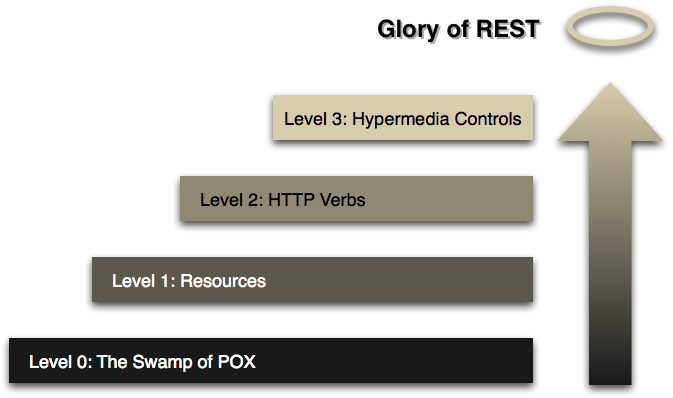
\includegraphics[width=0.8\textwidth]{rmm.png}
  \caption[Richardson Maturity Model]{Richardson Maturity Model \autocite{Fowler2010}}
  \label{fig:rmm}
\end{figure}

Een API is pas echt RESTful als het niveau 3 van het Richardson Maturity Model bereikt \autocite{Fowler2010}. HATEOAS is een belangrijk onderdeel van RESTful API design en wordt beschouwd als het hoogste niveau van volwassenheid. Echter is het implementeren van HATEOAS niet altijd eenvoudig en kan het extra complexiteit met zich meebrengen. Daarom zullen we in een volgend hoofdstuk grondig analyseren of de voordelen van HATEOAS opwegen tegen de nadelen in onze specifieke situatie.

\section{HATEOAS}

HATEOAS (Hypermedia as the Engine of Application State) is een belangrijk onderdeel van RESTful API design en vertegenwoordigt het hoogste niveau van volwassenheid volgens het Richardson Maturity Model (niveau 3) \autocite{Fowler2010}. Het kernidee achter HATEOAS is dat de server niet alleen data terugstuurt, maar ook hypermedia-links die de client informeren over welke acties mogelijk zijn op de opgevraagde data. Deze links fungeren als een soort "knoppen" in de API, die dynamisch veranderen afhankelijk van de status en rechten van de gebruiker.

\subsection{Werking van HATEOAS}

In een HATEOAS-API bevat elke response, naast de gevraagde data, ook links naar gerelateerde resources en mogelijke acties. Deze links worden meestal weergegeven in een gestandaardiseerd formaat, zoals JSON HAL (Hypertext Application Language) of Siren.

\begin{listing}[H]
  \begin{minted}{json}
  {
    "name": "Lars Salembier",
    "email": "lars.salembier@example.com",
    "_links": {
      "self": { "href": "/users/123" },
      "orders": { "href": "/users/123/orders" },
      "update": { "href": "/users/123", "method": "PUT" }
    }
  }
  \end{minted}
  \caption[Voorbeeld van een JSON HAL response]{Voorbeeld van een JSON HAL response met links naar gerelateerde resources en acties.}
  \label{lst:json_hal_example}
\end{listing}

In dit voorbeeld ziet u een JSON-object dat informatie over een gebruiker bevat. Naast de naam en het e-mailadres bevat het object ook een \texttt{links} sectie. Deze sectie bevat links naar gerelateerde resources, zoals de bestellingen van de gebruiker (\texttt{orders}), en mogelijke acties, zoals het bijwerken van de gebruikersgegevens (\texttt{update}). Elke link heeft een \texttt{href} attribuut dat de URL van de resource of actie specificeert, en optioneel een \texttt{method} attribuut dat de HTTP-methode aangeeft die gebruikt moet worden.

\subsection{Voordelen van HATEOAS}

Het gebruik van HATEOAS biedt verschillende voordelen:

\begin{itemize}
  \item \textbf{Loose Coupling:} Clients zijn minder afhankelijk van hardgecodeerde URI's. Als de serverstructuur verandert, hoeven de clients niet aangepast te worden, zolang de links correct blijven functioneren.
  \item \textbf{Ontdekkingsmogelijkheden:} Clients kunnen de API dynamisch ontdekken door de links in de responses te volgen. Dit vereenvoudigt de integratie en maakt de API meer zelfbeschrijvend.
  \item \textbf{Flexibiliteit:} De server kan de beschikbare acties en resources dynamisch aanpassen, zonder dat clients moeten worden bijgewerkt.
  \item \textbf{Documentatie:} HATEOAS kan de documentatie van de API vereenvoudigen, omdat de links zelf al informatie geven over de mogelijke acties en resources.
\end{itemize}

\subsection{Nadelen van HATEOAS}

\begin{itemize}
  \item \textbf{Complexiteit:} Het implementeren van HATEOAS kan complex zijn, vooral bij het ontwerpen van de API en het genereren van de juiste links.
  \item \textbf{Performance:} Het toevoegen van hypermedia-links aan elke response kan de performance van de API beïnvloeden, vooral bij grote datasets.
  \item \textbf{Overhead:} Het toevoegen van hypermedia-links aan elke response kan de grootte van de responses vergroten, wat kan leiden tot overhead.
  \item \textbf{Vendor Lock-in:} Het gebruik van HATEOAS kan leiden tot vendor lock-in, omdat clients afhankelijk zijn van de specifieke implementatie van de API.
  \item \textbf{Beveiliging:} Het toevoegen van hypermedia-links kan beveiligingsrisico's met zich meebrengen, zoals het blootstellen van gevoelige informatie.
  \item \textbf{Caching:} Het cachen van responses kan moeilijker zijn, omdat de links dynamisch gegenereerd worden.
\end{itemize}

\section{OpenAPI}

OpenAPI (voorheen bekend als Swagger) is een specificatie voor het beschrijven van RESTful API's in een machine-leesbaar formaat, meestal YAML of JSON \autocite{OpenAPIInitiative2021}. Het biedt een gestandaardiseerde manier om de structuur en functionaliteit van een API te documenteren, inclusief endpoints, parameters, request bodies, response bodies, authenticatiemethoden en meer. Deze documentatie kan vervolgens gebruikt worden voor diverse doeleinden, zoals het genereren van interactieve API documentatie, het automatisch genereren van client- en servercode, en het testen van de API.

\subsection{Structuur van een OpenAPI document}

Een OpenAPI document bevat verschillende secties die de API beschrijven:

\begin{itemize}
    \item \textbf{openapi:} De OpenAPI specificatie versie.
    \item \textbf{info:} Metadata over de API, zoals de titel, beschrijving en versie.
    \item \textbf{servers:} Een lijst van servers waar de API beschikbaar is.
    \item \textbf{paths:} De endpoints van de API, inclusief de ondersteunde HTTP-methoden en parameters.
    \item \textbf{components:} Herbruikbare componenten, zoals schemas (datatypes) en security schemes.
    \item \textbf{security:} De beveiligingsmechanismen die gebruikt worden door de API.
    \item \textbf{tags:} Tags om de API te categoriseren.
    \item \textbf{externalDocs:} Links naar externe documentatie.
\end{itemize}

\begin{listing}[H]
\begin{minted}{yaml}
openapi: 3.0.0
info:
  title: BrightEats API
  version: v1
paths:
  /orders:
    get:
      summary: Haal alle bestellingen op
      responses:
        '200':
          description: Lijst met bestellingen
          content:
            application/json:
              schema:
                type: array
                items:
                  $ref: '#/components/schemas/Order'
components:
  schemas:
    Order:
      type: object
      properties:
        id:
          type: integer
        description:
          type: string
\end{minted}
\caption[Voorbeeld van een OpenAPI document in YAML]{Voorbeeld van een OpenAPI document in YAML dat een endpoint beschrijft om bestellingen op te halen.}
\label{lst:openapi_example}
\end{listing}


\subsection{Tools voor OpenAPI}

Er zijn verschillende tools beschikbaar die werken met OpenAPI-documenten:

\begin{itemize}
  \item \textbf{Swagger UI:} Genereert interactieve documentatie waarmee gebruikers de API kunnen verkennen en testen.
  \item \textbf{Redoc:} Genereert statische documentatie in een aantrekkelijke en leesbare vorm.
  \item \textbf{OpenAPI Generator:} Genereert client- en servercode in verschillende programmeertalen op basis van een OpenAPI document.
  \item \textbf{Postman:} Ondersteunt het importeren en exporteren van OpenAPI-documenten en kan gebruikt worden voor het testen van de API.
\end{itemize}

\subsection{Voordelen van OpenAPI}

\begin{itemize}
  \item \textbf{Gestandaardiseerde documentatie:} OpenAPI biedt een gestandaardiseerde manier om API's te documenteren, waardoor de documentatie consistent en gemakkelijk te begrijpen is.
  \item \textbf{Automatische documentatiegeneratie:} Tools zoals Swagger UI en Redoc kunnen automatisch documentatie genereren op basis van een OpenAPI-document, waardoor de documentatie altijd up-to-date is.
  \item \textbf{Codegeneratie:} OpenAPI Generator kan client- en servercode genereren in verschillende programmeertalen, waardoor ontwikkeltijd wordt bespaard.
  \item \textbf{Testen:} OpenAPI-documenten kunnen gebruikt worden voor het automatisch testen van de API.
  \item \textbf{Samenwerking:} OpenAPI vergemakkelijkt de samenwerking tussen frontend- en backend-teams door een duidelijke en gedeelde specificatie van de API te bieden.
\end{itemize}

\subsection{Nadelen van OpenAPI}

\begin{itemize}
  \item \textbf{Leercurve:} Het leren schrijven en onderhouden van OpenAPI-documenten vereist enige inspanning.
  \item \textbf{Onderhoud:} OpenAPI documenten moeten up-to-date gehouden worden met de API, wat extra onderhoud vereist. Dit kan echter ook als een voordeel worden beschouwd, omdat het dwingt tot het consistent documenteren van de API.
\end{itemize}

\section{HATEOAS: Een evaluatie voor BrightAnalytics}

HATEOAS (Hypermedia as the Engine of Application State) vertegenwoordigt het hoogste niveau van volwassenheid binnen RESTful API design volgens het Richardson Maturity Model (niveau 3) \autocite{Fowler2010}. In dit hoofdstuk evalueren we de toepasbaarheid van HATEOAS binnen de specifieke context van BrightAnalytics. Hoewel HATEOAS theoretisch voordelen biedt, zullen we aantonen dat de implementatie ervan in onze situatie niet gerechtvaardigd is.

\subsection{Baten}

HATEOAS beidt clients de mogelijkheid om een API dynamisch te ontdekken en te navigeren zonder voorafgaande kennis van de URI-structuur. Elke response bevat hypermedia-links die de client informeren over de beschikbare acties en gerelateerde resources. Dit biedt potentiële voordelen zoals:

\begin{itemize}
  \item \textbf{Loose Coupling:} Clients zijn minder afhankelijk van hardgecodeerde URI's, waardoor de serverstructuur kan evolueren zonder directe impact op de clients.
  \item \textbf{Ontdekkingsmogelijkheden:} Clients kunnen de API dynamisch verkennen door de aangeboden links te volgen.
  \item \textbf{Flexibiliteit:} De server kan de beschikbare acties en resources dynamisch aanpassen.
\end{itemize}

\subsection{Kosten}

Een cruciaal aspect van onze situatie is dat de te ontwikkelen API's uitsluitend intern gebruikt zullen worden binnen BrightAnalytics. Dit betekent dat de development teams directe toegang hebben tot uitgebreide documentatie en effectief kunnen communiceren over de API-structuur. De noodzaak voor de ontdekkingsmogelijkheden die HATEOAS biedt, wordt hierdoor sterk gereduceerd.

\bigskip

De implementatie van HATEOAS brengt aanzienlijke kosten met zich mee, die in onze context niet opwegen tegen de beperkte voordelen.

\bigskip

Het genereren en beheren van hypermedia-links introduceert extra complexiteit in de ontwikkeling van de API. Dit vereist een doordachte implementatie en grondig testen om de correctheid en consistentie van de links te garanderen.

\bigskip

Het toevoegen van hypermedia-links aan elke response vergroot de hoeveelheid data die verzonden moet worden. Dit kan een negatieve impact hebben op de performance, met name bij grote datasets.

\bigskip

Gezien de interne context en de reeds aanwezige communicatiekanalen binnen de development teams, is de meerwaarde van HATEOAS beperkt. De kosten van implementatie en onderhoud wegen niet op tegen de minimale winst in ontdekkingsmogelijkheden.

\bigskip

De ontwikkeling van de API's zal gepaard gaan met uitgebreide documentatie gebaseerd op de OpenAPI specificatie. Met behulp van tools zoals Swagger UI of Redoc zal deze documentatie interactief en gemakkelijk toegankelijk zijn voor alle betrokken developers. Dit biedt een effectief alternatief voor de ontdekkingsmogelijkheden van HATEOAS, zonder de bijbehorende complexiteit en overhead.

\subsection{Conclusie}

Gezien de interne context van de API's bij BrightAnalytics en de beschikbaarheid van uitgebreide OpenAPI documentatie, concluderen we dat de implementatie van HATEOAS niet gerechtvaardigd is. De kosten en complexiteit wegen niet op tegen de beperkte voordelen. Daarom kiezen we ervoor om HATEOAS niet te implementeren in onze API's.

\section{RESTful API best practices en de Zalando Guidelines}

Het ontwerpen en implementeren van hoogwaardige, onderhoudbare en schaalbare RESTful API's vereist het volgen van best practices. Hoewel een gedetailleerde bespreking van alle best practices buiten het bestek van deze literatuurstudie valt, erkennen we het belang ervan en zullen we een set specifieke richtlijnen opstellen tijdens de ontwikkelingsfase van onze API's. Hierbij zullen we ons baseren op de uitgebreide \textit{Zalando RESTful API Guidelines} \autocite{ZAG2024}.

\subsection{De Zalando RESTful API Guidelines}

De Zalando RESTful API Guidelines bieden een uitgebreid framework voor het ontwerpen en ontwikkelen van RESTful API's. Deze guidelines behandelen een breed scala aan onderwerpen, waaronder:

\begin{itemize}
  \item \textbf{URI Design:} Richtlijnen voor het creëren van consistente, leesbare en betekenisvolle URI's.
  \item \textbf{HTTP Methoden:} Correct gebruik van HTTP methoden (GET, POST, PUT, PATCH, DELETE) en hun semantische betekenis.
  \item \textbf{Status Codes:} Gebruik van de juiste HTTP status codes om de uitkomst van requests te communiceren.
  \item \textbf{Dataformaten:} Richtlijnen voor het gebruik van de juiste dataformaten.
  \item \textbf{Versionering:} Strategieën voor het beheren van API versies en het waarborgen van backward compatibility.
  \item \textbf{Foutbehandeling:} Best practices voor het afhandelen en rapporteren van fouten.
  \item \textbf{Authenticatie en Autorisatie:} Beveiligingsmechanismen voor het beschermen van de API.
  \item \textbf{Documentatie:} Het belang van duidelijke en complete API documentatie.
  \item \textbf{Paginering:} Technieken voor het efficiënt verwerken van grote datasets.
  \item \textbf{Filtering en Sortering:} Mogelijkheden voor clients om data te filteren en te sorteren.
\end{itemize}

De Zalando RESTful API Guidelines bieden een waardevolle bron van best practices en richtlijnen voor het ontwerpen van RESTful API's. We zullen deze guidelines gebruiken als basis voor het opstellen van onze eigen set richtlijnen tijdens de ontwikkeling van de Bright\-Eats API.

\section{Implementatie met Laravel en Vue.js}

Dit hoofdstuk beschrijft de gekozen technologieën voor de backend en frontend ontwikkeling, namelijk Laravel en Vue.js, en hoe de concepten van RESTful API design en OpenAPI daarop worden toegepast.

\subsection{Laravel als backend framework}

Laravel is een populair PHP framework dat zich uitstekend leent voor het ontwikkelen van robuuste en schaalbare webapplicaties, inclusief RESTful API's. We kiezen voor Laravel vanwege de volgende redenen \autocite{Laravel}:

\begin{itemize}
  \item \textbf{MVC Architectuur:} Laravel's Model-View-Controller architectuur bevordert een gestructureerde en modulaire codebase, wat de ontwikkeling en onderhoudbaarheid van API's vereenvoudigt.
  \item \textbf{Eloquent ORM:} De Eloquent ORM (Object-Relational Mapper) maakt het eenvoudig om te interageren met databases en data te manipuleren.
  \item \textbf{Routing:} Laravel biedt een flexibel en krachtig routing systeem voor het definiëren van API endpoints.
  \item \textbf{Middleware:} Middleware in Laravel kan gebruikt worden voor taken zoals authenticatie, autorisatie, logging en request validatie.
  \item \textbf{Testing:} Laravel biedt uitgebreide mogelijkheden voor het testen van API's.
  \item \textbf{Community en Documentatie:} Laravel heeft een grote en actieve community en uitgebreide documentatie, wat de ontwikkeling vergemakkelijkt.
\end{itemize}

\subsubsection{RESTful API's in Laravel}

Laravel biedt ingebouwde ondersteuning voor het ontwikkelen van RESTful API's. Resources kunnen worden gedefinieerd met behulp van resource controllers en routes.

\begin{listing}[H]
\begin{minted}{php}
  use App\Models\Product;
  use Illuminate\Http\Request;
  use App\Http\Resources\ProductResource;
  
  class ProductController extends Controller
  {
    public function index()
    {
      return ProductResource::collection(Product::all());
    }

    public function show(Product $product)
    {
      return new ProductResource($product);
    }

    public function store(Request $request)
    {
      $validated = $request->validate([
        'name' => 'required|max:255',
        'price' => 'required|numeric',
      ]);

      $product = Product::create($validated);

      return new ProductResource($product);
    }

    // ... update, destroy methods ...
  }
\end{minted}
\caption[Voorbeeld van een Laravel resource controller]{Voorbeeld van een Laravel resource controller voor het beheren van producten.}
\label{lst:laravel_controller}
\end{listing}

\subsection{Vue.js als frontend framework}

Vue.js is een progressief JavaScript framework dat ideaal is voor het bouwen van interactieve user interfaces \autocite{VueJS}. We kiezen voor Vue.js vanwege:

\begin{itemize}
  \item \textbf{Component-gebaseerde architectuur:} Vue.js stimuleert het ontwikkelen van herbruikbare componenten, wat de codebase overzichtelijker en onderhoudbaarder maakt.
  \item \textbf{Reactiviteit:} Vue.js' reactieve data binding zorgt ervoor dat de user interface automatisch wordt bijgewerkt wanneer de data verandert.
  \item \textbf{Eenvoudige integratie:} Vue.js kan gemakkelijk geïntegreerd worden met andere libraries en frameworks.
  \item \textbf{Performance:} Vue.js is lightweight en performant.
  \item \textbf{Community en Documentatie:} Net als Laravel heeft Vue.js een grote en actieve community en uitgebreide documentatie.
\end{itemize}

\subsubsection{Consumptie van de API in Vue.js}

Vue.js-applicaties kunnen de Laravel API consumeren met behulp van HTTP clients zoals Axios of de ingebouwde Fetch API. Data opgehaald van de API kan vervolgens gebruikt worden om de user interface dynamisch te vullen.

\begin{listing}[H]
\begin{minted}{javascript}
  import axios from 'axios';

  export default {
  data() {
    return {
      products: [],
    };
  },
  mounted() {
    axios.get('/api/products')
      .then(response => {
        this.products = response.data.data;
      })
      .catch(error => {
        console.error(error);
      });
  },
  };
\end{minted}
\caption[Voorbeeld van het ophalen van data van een Laravel API in Vue.js]{Voorbeeld van het ophalen van data van een Laravel API in Vue.js met behulp van Axios.}
\label{lst:vue_axios}
\end{listing}

\subsection{OpenAPI integratie}

OpenAPI zal een centrale rol spelen in de ontwikkeling van onze API's. We zullen een OpenAPI-document creëren dat de API volledig beschrijft. Dit document zal dienen als basis voor:

\begin{itemize}
  \item \textbf{Documentatie:} Automatische generatie van interactieve documentatie met behulp van tools zoals Swagger UI.
  \item \textbf{Client code generatie:} Mogelijkheid om client code te genereren in verschillende talen.
  \item \textbf{Server side validatie:} Validatie van requests en responses op basis van het OpenAPI schema.
  \item \textbf{Testing:} Automatische tests genereren op basis van het OpenAPI document.
\end{itemize}

Door OpenAPI te integreren in ons ontwikkelproces, zorgen we voor een consistente, goed gedocumenteerde en gemakkelijk te onderhouden API.

\begin{listing}[H]
\begin{minted}{yaml}
paths:
  /products:
    get:
      summary: Get all products
      responses:
        '200':
          description: A list of products
          content:
            application/json:
              schema:
                type: object
                properties:
                  data:
                    type: array
                    items:
                      $ref: '#/components/schemas/Product'
components:
  schemas:
    Product:
      type: object
      properties:
        id:
          type: integer
          readOnly: true
        name:
          type: string
        price:
          type: number
          format: float
\end{minted}
\caption[Voorbeeld van een OpenAPI document in YAML]{Voorbeeld van een OpenAPI document in YAML dat een endpoint beschrijft om producten op te halen.}
\label{lst:openapi_example_resource}
\end{listing}

\section{Conclusie}

Deze literatuurstudie heeft een overzicht geboden van de belangrijkste concepten en technologieën die relevant zijn voor het ontwikkelen van robuuste, schaalbare en goed gedocumenteerde RESTful API's, met specifieke aandacht voor de context van BrightAnalytics en hun bestaande technologie stack. We begonnen met een inleiding tot API's in het algemeen, waarna we de principes van RESTful API design hebben geanalyseerd, inclusief de zes belangrijkste principes (Client-Server, Stateless, Cacheable, Uniform Interface, Layered System en Code-On-Demand), HTTP methoden, status codes en het resource-gebaseerde karakter van REST.

\bigskip

Vervolgens introduceerden we het Richardson Maturity Model, dat de volwassenheid van RESTful API's beschrijft, met speciale aandacht voor HATEOAS. Na een grondige evaluatie van de voor- en nadelen van HATEOAS, in combinatie met de specifieke context van BrightAnalytics - interne API's en een nadruk op heldere documentatie - concludeerden we dat de implementatie van HATEOAS voor dit project niet de meest efficiënte aanpak is. De complexiteit en overhead wegen niet op tegen de beperkte voordelen in onze situatie. Deze beslissing wordt versterkt door onze keuze voor OpenAPI, waarmee we uitgebreide en interactieve documentatie zullen genereren, wat de noodzaak voor de ontdekkingsaspecten van HATEOAS minimaliseert.

\bigskip

OpenAPI vormt een kerncomponent in onze API-ontwikkelingsstrategie. Door een OpenAPI-document te creëren dat de API volledig beschrijft, waarborgen we consistente documentatie, automatische codegeneratie, server-side validatie en geautomatiseerd testen. Dit bevordert de kwaliteit, onderhoudbaarheid en schaalbaarheid van onze API's. De integratie van OpenAPI, gecombineerd met de techstack van BrightAnalytics (Laravel en Vue.js), optimaliseert ons ontwikkelproces.

\bigskip

Ten slotte benadrukten we het belang van best practices voor API-ontwikkeling. Een gedetailleerde beschrijving hiervan valt buiten het bestek van deze literatuurstudie, maar tijdens de ontwikkeling zullen we specifieke richtlijnen formuleren, gebaseerd op de Zalando RESTful API Guidelines. Dit framework biedt een solide basis voor het ontwerpen en implementeren van RESTful API's, waarmee we de consistentie, betrouwbaarheid en schaalbaarheid van onze API's willen verhogen.
